% Chapter 1

\chapter{Organization of the project} % Main chapter title

\label{Chapter2} % For referencing the chapter elsewhere, use \ref{Chapter1} 

%----------------------------------------------------------------------------------------

We can firstly explain how this project is organized:

\section{The role of the designer and the users}
In this design process the interaction between designer and users is very strict: in fact for about 2 months, divided in blocks of more of less 2 weeks, the designer has worked together directly with the users. 

It is interesting to note that the domain in which this application works is quite complex and different from the domains in which the designer is specialized, so, some periods of work directly with the users are necessary to let the developer understand better how does the domain works.
This period of time allowed the designer to understand better how exactly the work processes take place, and what are the needs of the users. 
It is important to precise that this kind of users is quite particular: their education level is very high (almost all of them have a Phd), and their need are very specialized (related with the physics research world).

In this design process we can identify 3 main actors: 
\begin{enumerate}

\item
The designer, who produced the web interface (gAn Web)

\item 
Two pilot users (university professors in Brescia), that are also co-developer of the application behind this interface (gAn). So they act both the role of the users, and the role of the supervisors. 

\item A group of users (around 10-12) in Geneva. This main group is used for the final testing of the application.
 
\end{enumerate}

\section{The stages of the project}

The design process can be also divider in three stages:

\begin{figure}[H]
\centering
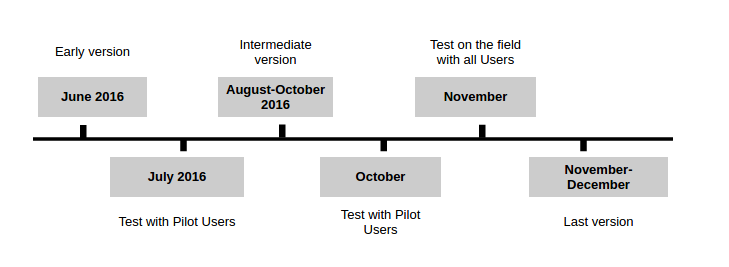
\includegraphics[scale=0.5]{TimeLine.png} 
\caption{An overview of the timeline of the project}
\end{figure}


\begin{enumerate}

% 1
\item An early stage, more simple, with basic functionalities, just to investigate what are the best ways to implement the functionalities and to test with a little group of pilot-users (two) if this software can really be useful and which functionalities are really important; The goal of this stage is to give an initial direction to the development and to improve the designer's knowledge of the domain. At the end of this stage, the test with the two pilot users helps to correct the way.

% 2
\item An intermediate stage, more complex, with some advanced functionalities obtained listening the request of the pilot users. This version is installed in the AEgIS control room and the users use it. 
The designer needs at this point to execute some test with the maximum possible number of users to understand if the product is acceptable and useful (and how to improve it). 

In this stage the test with the users are splitted in two blocks:  
The first block is another test with the pilot users, that are present in all the stages (they are, as well as users, also supervisors), and their hints are applied before let the group of generic users work with the application;
The second block is a test with a big group of users that works with the application in the AEgIS Control Room.

The tests with the users show a lot of useful information and allow the developer to find a big group of problems: the solutions to these problems give the birth at the final version. 

% 3
\item
The third stage is the final stage. At this point the application is modified to accord the observations of the users. It is important to notice that the third stage (the last one) is a never-finished stage: the needs of the users are permanently changing and evolving, the application is designed to be adaptable, and to try to satisfy the unknown needs of future users.

\end{enumerate}

According to this division we can organize the following chapters in this way:
each chapter is related to a stage of the development.
For each of the three stages of the development this document will explain:

\begin {enumerate}

\item
The requirements of the web interface.

\item
The functional analysis of the requirements through some expected scenarios

\item
The the resulting prototyping (and implementation)  

\end {enumerate} 

